\section{eo\-Stoch\-Tournament\-Truncate$<$ EOT $>$ Class Template Reference}
\label{classeo_stoch_tournament_truncate}\index{eoStochTournamentTruncate@{eoStochTournamentTruncate}}
a truncate class based on a repeated deterministic (reverse!) tournament To be used in SSGA-like replacements (e.g.  


{\tt \#include $<$eo\-Reduce.h$>$}

Inheritance diagram for eo\-Stoch\-Tournament\-Truncate$<$ EOT $>$::\begin{figure}[H]
\begin{center}
\leavevmode
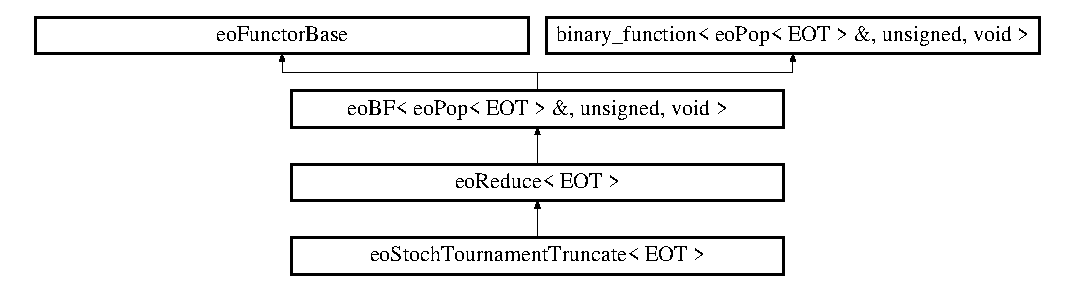
\includegraphics[height=3.45679cm]{classeo_stoch_tournament_truncate}
\end{center}
\end{figure}
\subsection*{Public Member Functions}
\begin{CompactItemize}
\item 
{\bf eo\-Stoch\-Tournament\-Truncate} (double \_\-t\_\-rate)\label{classeo_stoch_tournament_truncate_a0}

\item 
void {\bf operator()} ({\bf eo\-Pop}$<$ {\bf EOT} $>$ \&\_\-newgen, unsigned \_\-newsize)\label{classeo_stoch_tournament_truncate_a1}

\begin{CompactList}\small\item\em The pure virtual function that needs to be implemented by the subclass. \item\end{CompactList}\end{CompactItemize}
\subsection*{Private Attributes}
\begin{CompactItemize}
\item 
double {\bf t\_\-rate}\label{classeo_stoch_tournament_truncate_r0}

\end{CompactItemize}


\subsection{Detailed Description}
\subsubsection*{template$<$class EOT$>$ class eo\-Stoch\-Tournament\-Truncate$<$ EOT $>$}

a truncate class based on a repeated deterministic (reverse!) tournament To be used in SSGA-like replacements (e.g. 

see {\bf eo\-SSGAStoch\-Tournament\-Replacement}{\rm (p.\,\pageref{classeo_s_s_g_a_stoch_tournament_replacement})}) 



Definition at line 236 of file eo\-Reduce.h.

The documentation for this class was generated from the following file:\begin{CompactItemize}
\item 
eo\-Reduce.h\end{CompactItemize}
